\section{Operational Hardening and Infrastructure}\label{sec:security-hardening}

To ensure the resilience of the CFI-Care platform, we implemented a series of operational hardening measures across the network, application, and container layers. 
These configurations form a multi-layered defense against common attack vectors.


\subsection{Perimeter Firewall and System Access Plan}\label{sec:security-firewall}
We placed an OPNsense perimeter firewall at the network edge, providing WAN and LAN interfaces and performing NAT for internal services. 
The firewall enforces a minimal exposure policy: only HTTPS (443) is forwarded to the internal Nginx reverse proxy, 
the management GUI (Whose Main dashboard can be seen in Fig~\ref{fig:opnsense-lobby} ) is restricted to a dedicated management VLAN, and administrative access is additionally protected with MFA and off-host encrypted backups.
This flow can be seen in Figure~\ref{fig:sys-access-plan} \newline

\textbf{Operational controls:}

\begin{itemize}
    \item \textbf{Management access}: GUI restricted to the management network only and protected by MFA.
    \item \textbf{Public exposure:} only the reverse proxy (Nginx) is reachable from WAN on TCP/443.
    \item \textbf{Backups}: OPNsense configuration exports are encrypted and stored off-host.
\end{itemize}

\begin{figure}[H]
    \centering
    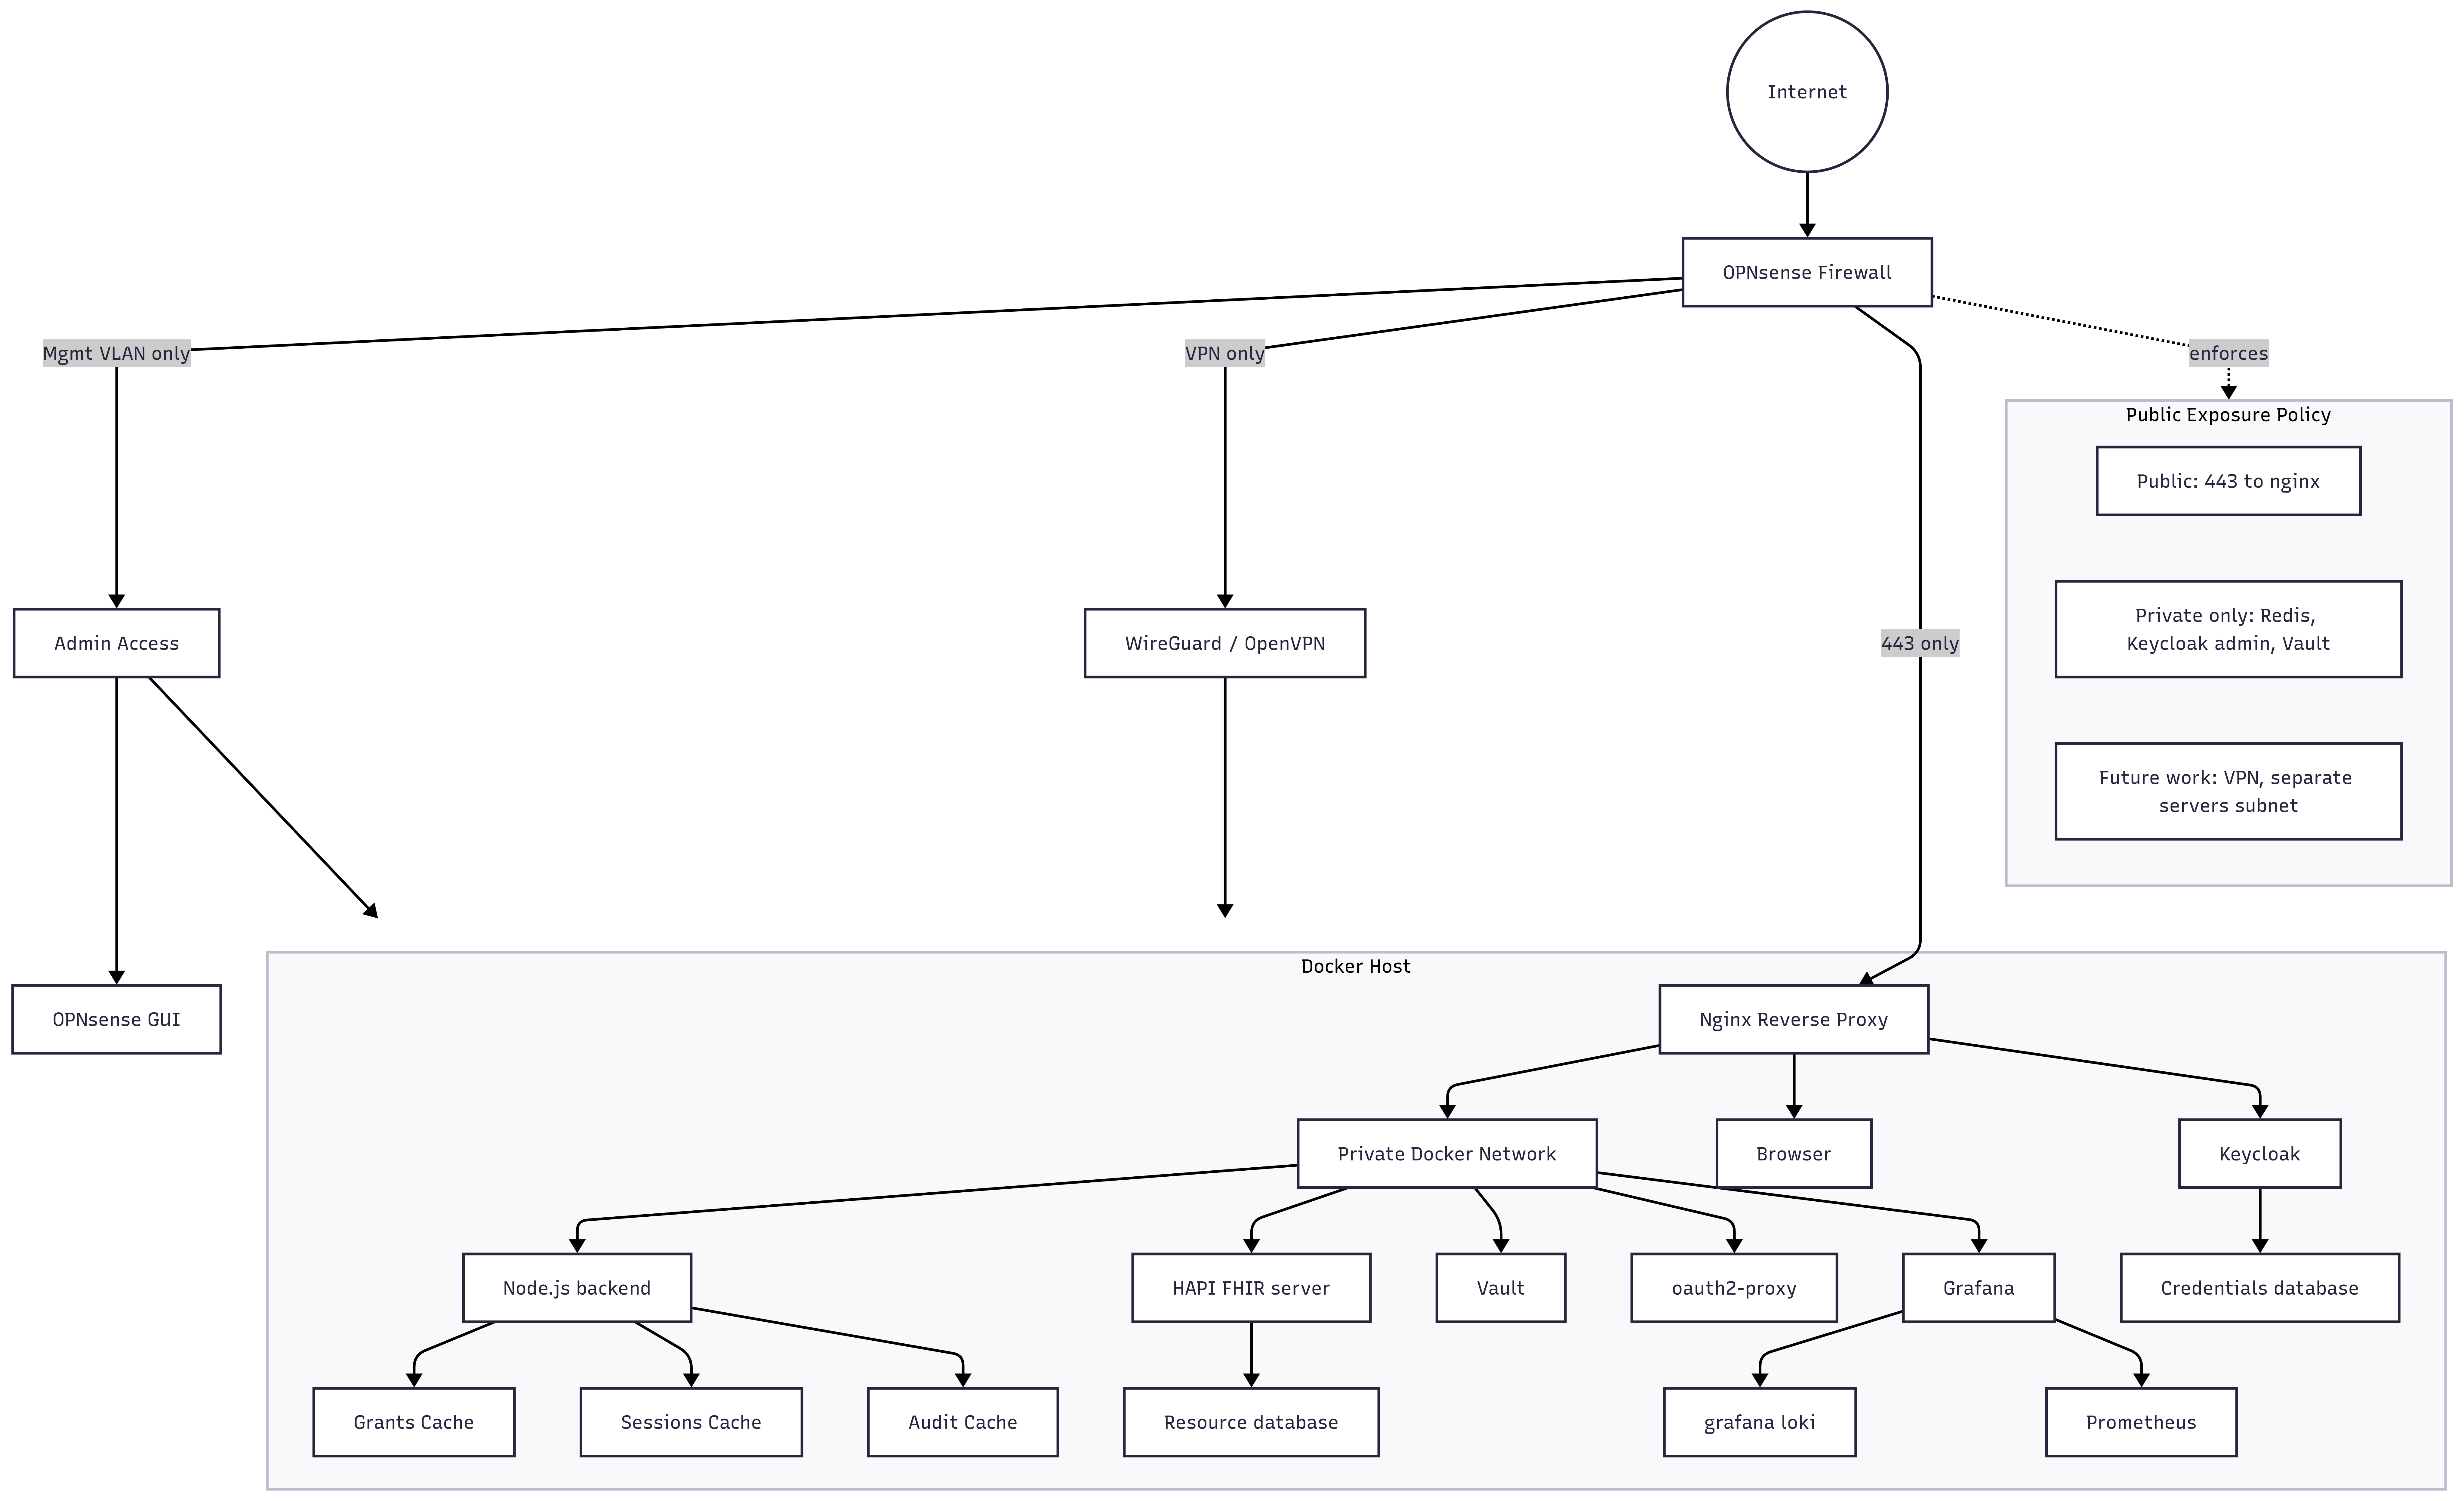
\includegraphics[width=0.95\linewidth]{Security/images/System-access-plan.png}
    \caption{System Access diagram}
    \label{fig:sys-access-plan}
\end{figure}

\begin{figure}[H]
    \centering
    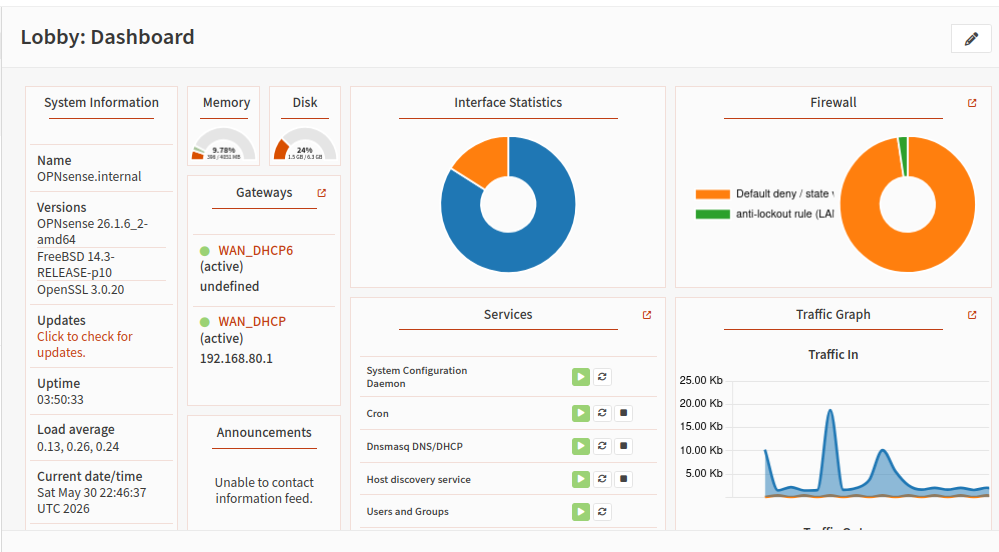
\includegraphics[width=1.0\linewidth]{Security/images/Firewall Dashboard.png}
    \caption{OPNsense Perimeter Administration Interface: Active validation environment mapping network interface distribution, load profiles, and system operational states.}
    \label{fig:opnsense-lobby}
\end{figure}

\subsection{Infrastructure Security and Gateway Configuration}

The Nginx API Gateway serves as the single entry point for all traffic, acting as a security buffer between external clients and internal microservices.

\paragraph{Transport Layer Security (TLS)}
TLS is terminated at the Nginx edge. All traffic on port 80 is forcibly redirected to port 443, 
ensuring that every byte in transit is encrypted. 
Since we're more focused on the development phase, self-signed certificates are utilized, with a planned transition to CA-signed certificates (Let’s Encrypt) for production.

\paragraph{Proxy Hardening and Header Management}
Nginx is configured to set \newline \texttt{X-Forwarded-*} headers, allowing the internal BFF service to correctly identify client IP addresses and protocol types. 
This is essential for the \texttt{trust proxy} setting in Express, which ensures that session cookies are only marked as \texttt{Secure} when a valid HTTPS connection is detected.
Also, to ensure architectural integrity and prevent host-header injection attacks, the gateway is configured to preserve the Host header while sanitizing incoming proxy headers, which ensures that the BFF reliably identifies the request origin, maintaining a consistent security context across the infrastructure.

\subsection{Application Layer Hardening}

% The Backend-for-Frontend (BFF) employs the \textbf{Helmet} middleware suite to enforce strict browser-side security policies through HTTP headers:
The application runtime security model hardens the \ac{BFF} by sealing the client-browser execution environment through its constraining middleware

\begin{itemize}
%     \item \textbf{Content Security Policy (CSP) \& Frame Options:} \newline \texttt{Content-Security-Policy} and \texttt{X-Frame-Options} (SAMEORIGIN) , significantly reduce the surface area for \ac{XSS}, clickjacking attacks and unauthorized framing.
%     \item \textbf{HSTS:} \texttt{Strict-Transport-Security} mandates HTTPS for a duration of one year, preventing protocol downgrade attacks.
%     \item \textbf{CORS:} Configured to restrict \ac{API} access strictly to the Angular frontend's origin. By enabling \texttt{withCredentials: true}, the system supports secure, cross-origin cookie transmission without exposing tokens to the client-side JavaScript.
% \end{itemize}

    \item \textbf{Downstream Policy Enforcement:} Security header mutations managed via Helmet mandate strict runtime isolation, injecting deterministic \texttt{SAMEORIGIN} framing definitions and multi-layered context restrictions to prevent hostile browser-side script execution.
    \item \textbf{Transport Mandates:} Downstream clients are bound to continuous transport security using long-duration \texttt{Strict-Transport-Security} (HSTS) responses, effectively eliminating protocol downgrading risks.
    \item \textbf{Origin Pinning:} \ac{CORS} configuration explicitly mirrors and isolates valid Angular UI boundaries, using a strict origin policy alongside the \texttt{withCredentials} flag to prevent client-side script interception of application token assets.
\end{itemize}

\subsection{Secrets Management}
Secrets management is centralized using HashiCorp Vault service and Vault agents. 
Vault houses environment secrets and role-based credentials for Keycloak, Node.js, HAPI FHIR and oauth2-proxy servers. 
Containerized Vault agents render templated environment files at startup and expose only the minimal runtime secrets to each service. 
This reduces secret exposure, enables the ability to later automate rotation via Vault policies 
and provides a clearer operational separation between secret storage and application logic
Vault architecture can be seen in the following diagram \ref{fig:vault-arch}

\begin{figure}[H]
    \centering
    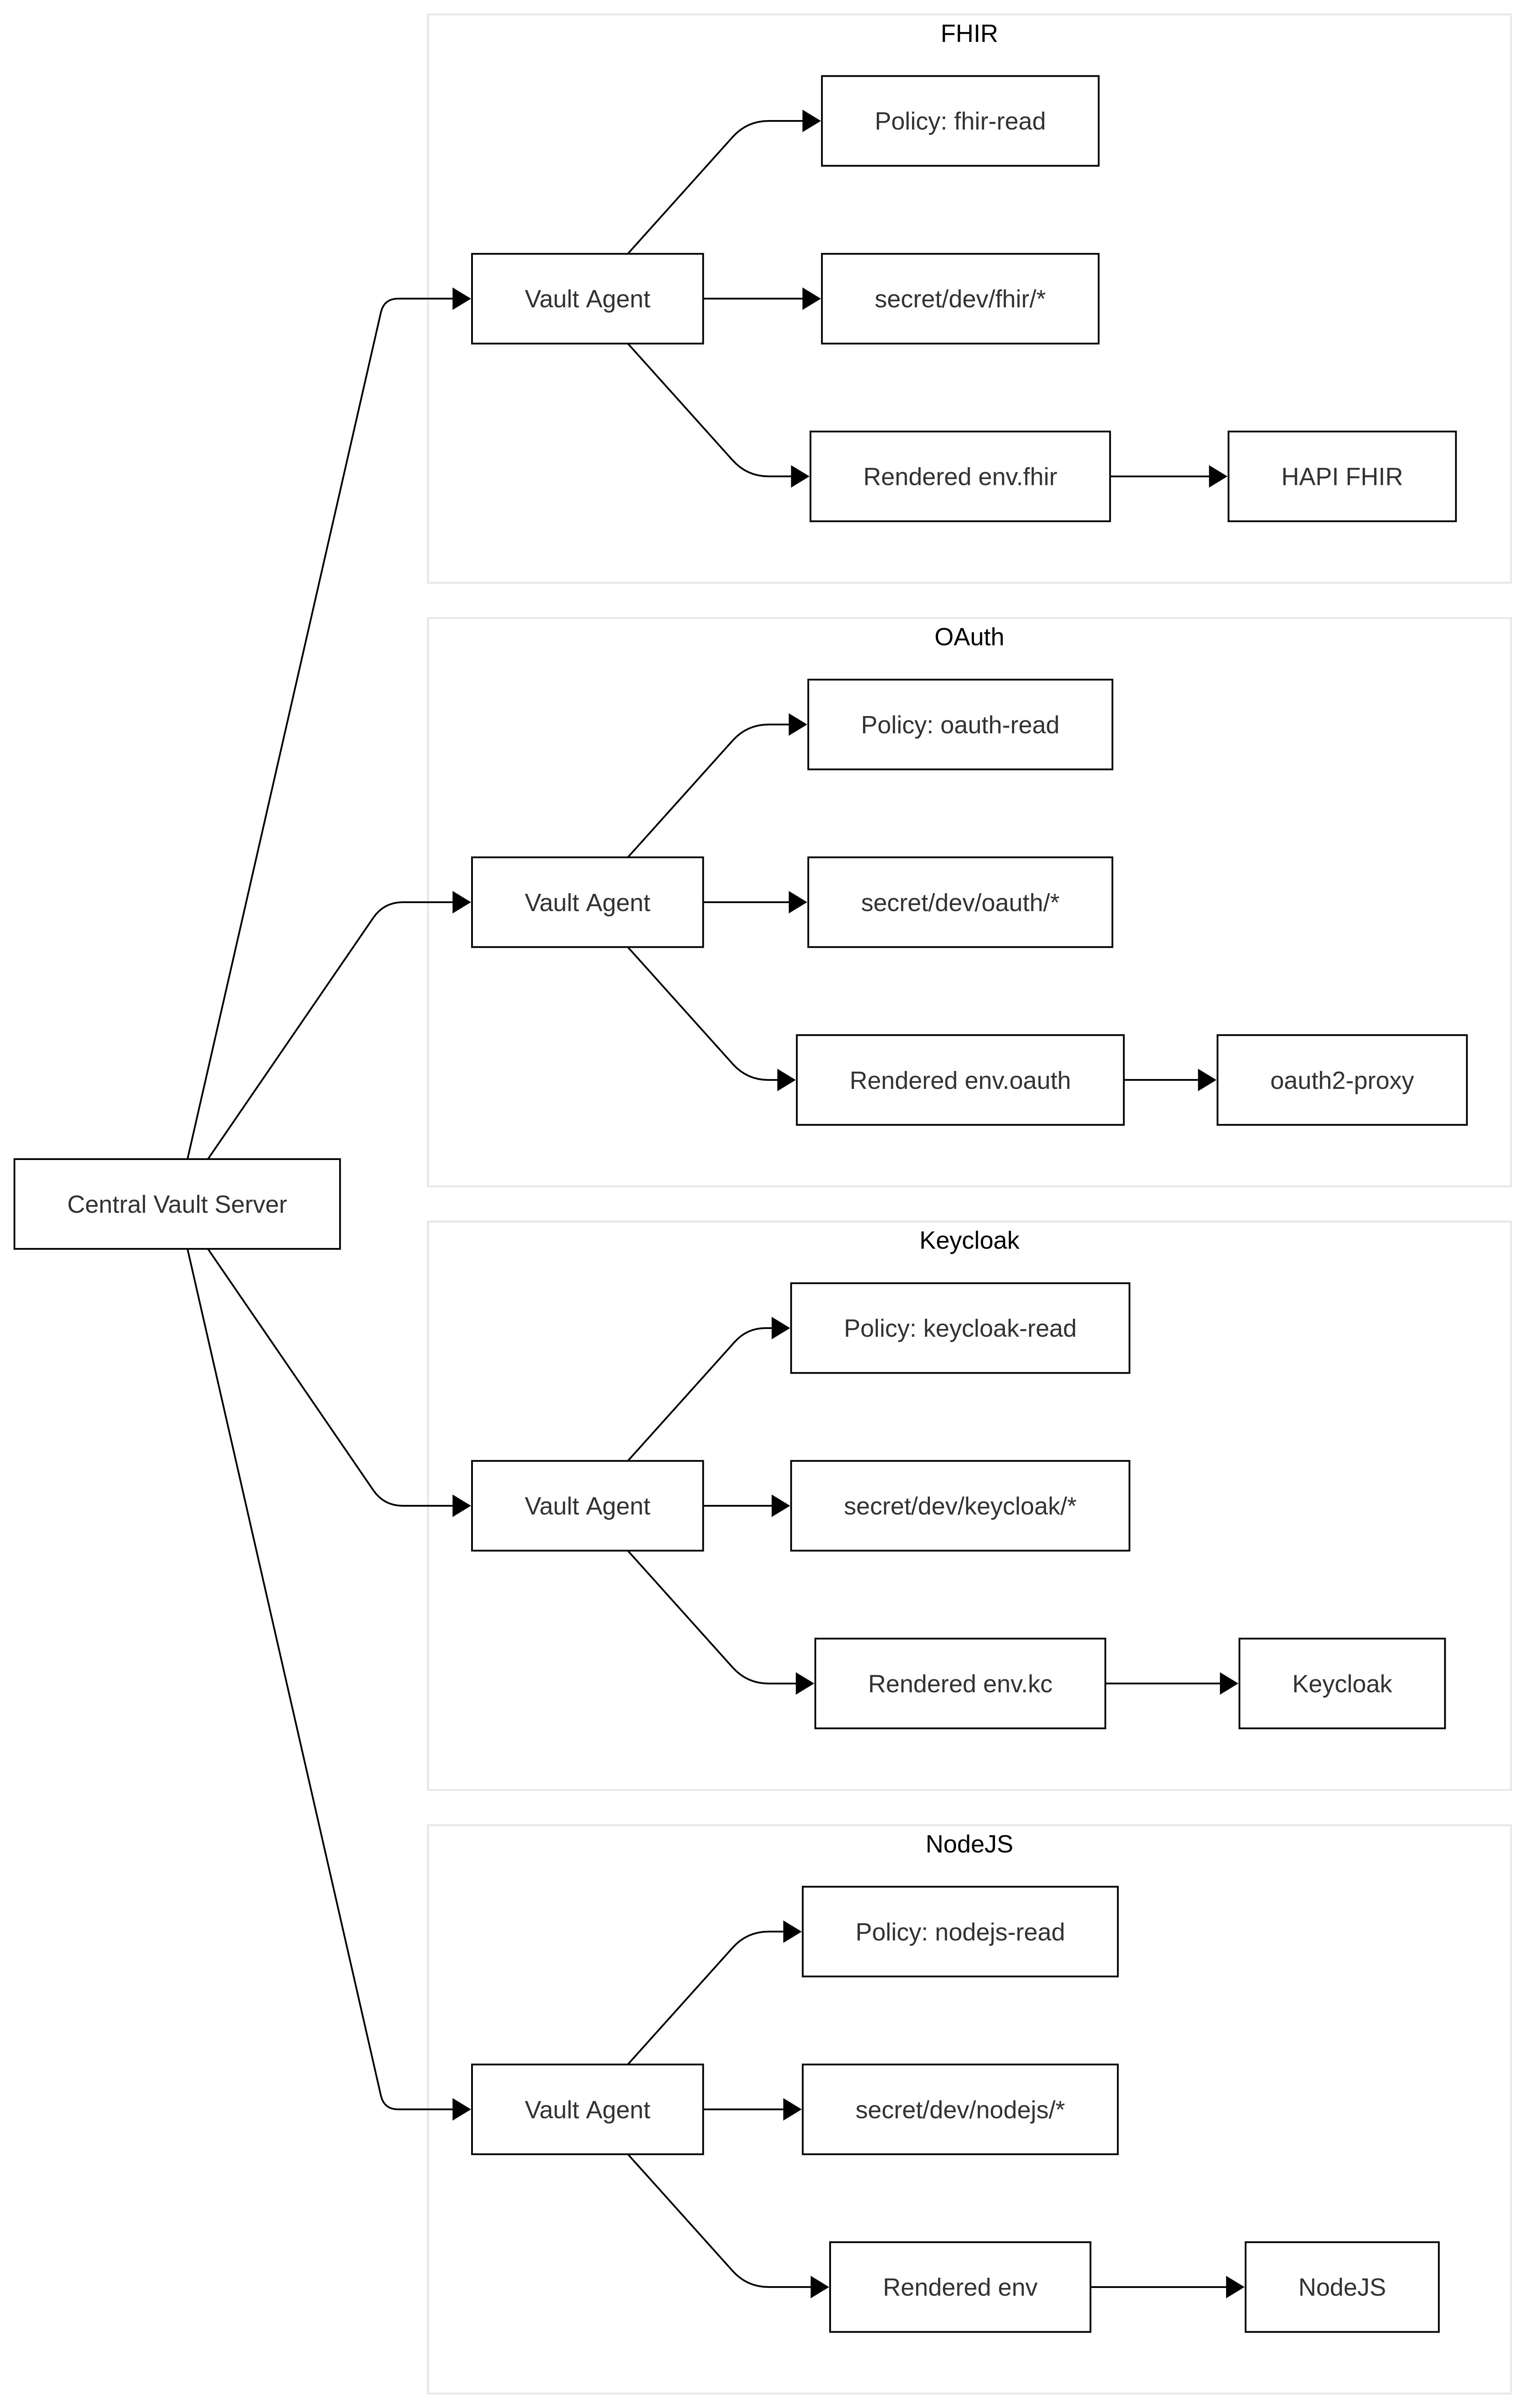
\includegraphics[width=0.7\linewidth]{Security/images/vault-plan.png}
    \caption{Vault architecture diagram}
    \label{fig:vault-arch}
\end{figure}

\subsection{Audit Logging and Observability}

Accountability is maintained through a dedicated \textbf{Security Event Logger} integrated into the BFF.

\paragraph{Audit Trail Design}
All critical authentication and authorization events are persisted in a Redis-backed \textbf{Audit Store}. Each entry captures the timestamp, User ID, Client IP, and User-Agent.
\paragraph{Retention and Analysis}
Entries are stored in sorted sets with a 90-day retention policy. This structured log allows for forensic analysis and satisfies privacy regulations by providing a transparent history of sensitive data access.

\paragraph{Visualization}
we integrated a lightweight observability stack composed of Prometheus (metrics), Grafana (visualisation), and Loki (log indexing). 
Audit events retained in Redis are forwarded to Loki via the Loki push API, and displayed as ordered logs in its Grafana dashboard (Seen in Fig~\ref{fig:audit-raw-streams}) . 
Prometheus scrapes application metrics exposed at specific endpoints and feeds its dashboard for real-time statistical analysis (As seen in Fig~\ref{fig:audit-metrics})

\begin{figure}[H]
    \centering
    % \begin{subfigure}[b]
        \centering
        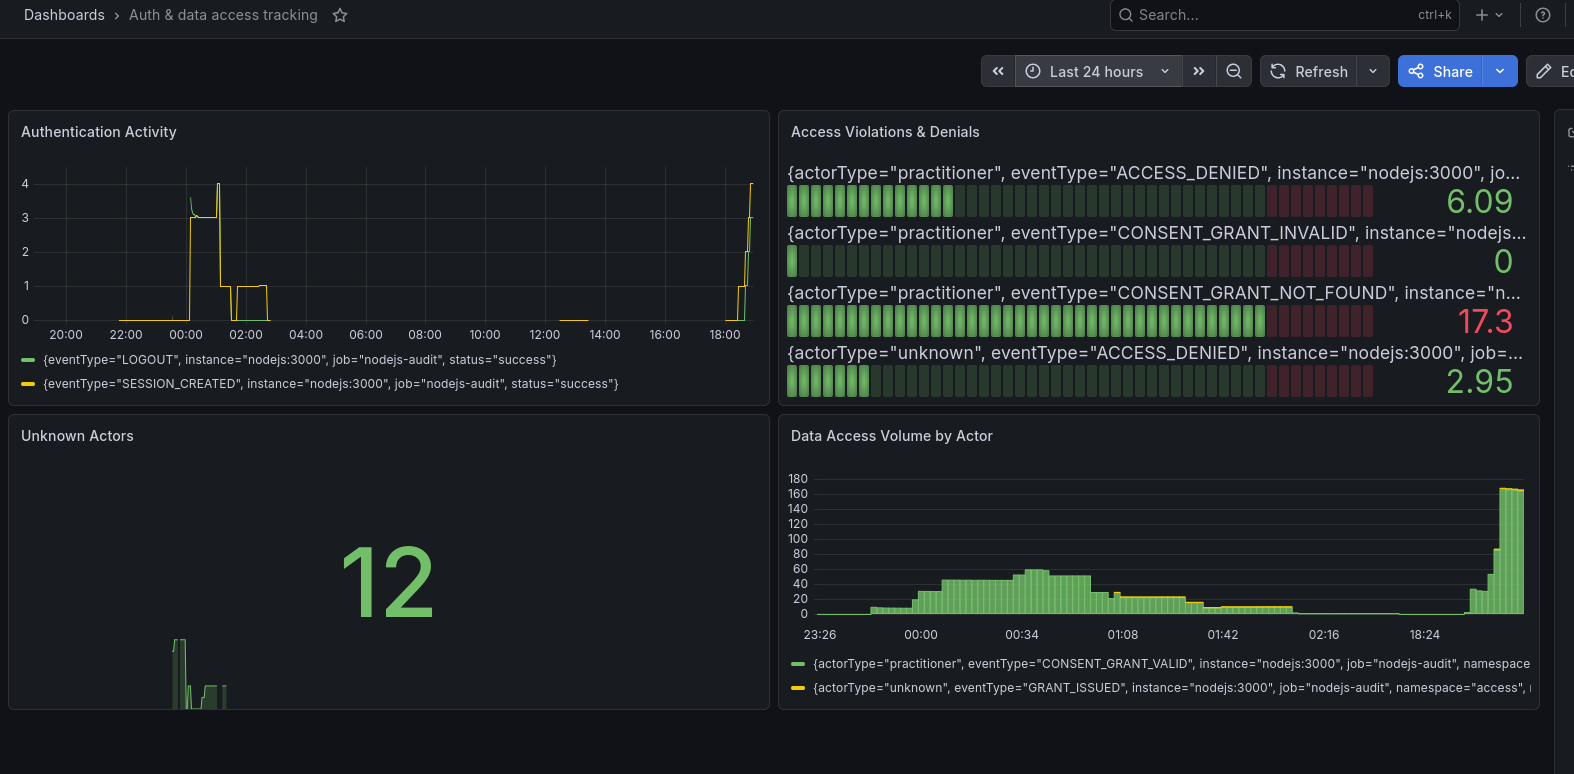
\includegraphics[width=0.85\linewidth]{Security/images/audit/metrics.png}
        \caption{Grafana Security Dashboard mapping runtime volumetric authorization metrics, credential access violations, and structural log alerts.}
        \label{fig:audit-metrics}
    % \end{subfigure}
\end{figure}
    \vspace{0.3cm}
\begin{figure}[H] 
    % \begin{subfigure}[b]
        \centering
        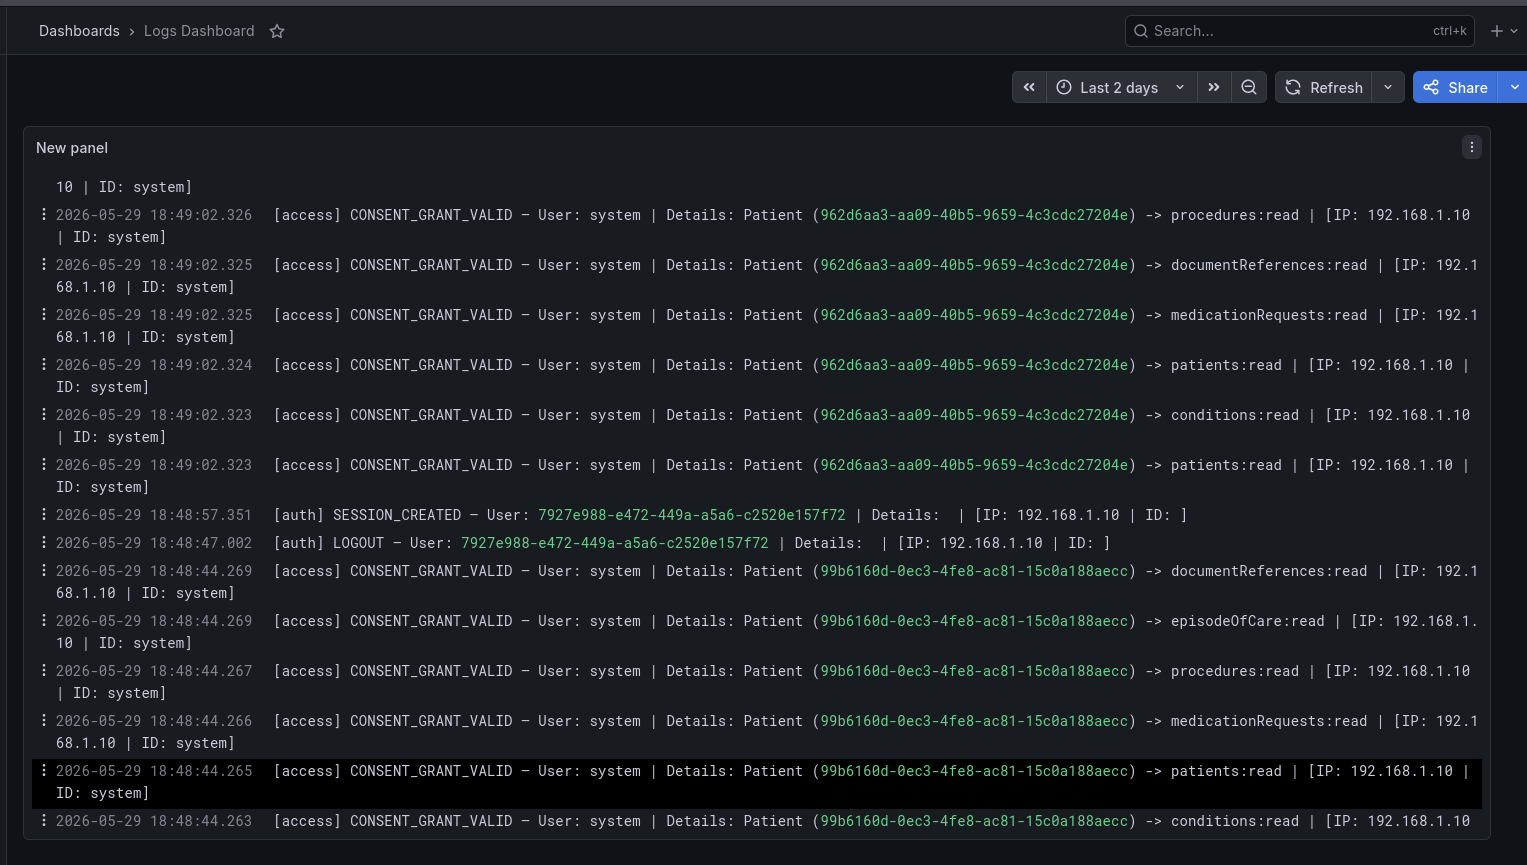
\includegraphics[width=0.85\linewidth]{Security/images/audit/logs.png}
        \caption{Structured security log streams containing granular authorization events, runtime timestamps, and user identifiers.}
        \label{fig:audit-raw-streams}
    % \end{subfigure}
    % \caption{Unified Security Audit Monitoring Framework: Aggregated telemetry validating system access trends and real-time transaction tracking.}
    % \label{fig:grafana-audit-suite}
\end{figure}


\subsection{Container and Network Isolation}

The deployment architecture utilizes Docker Compose to enforce network-level isolation between services.
\begin{itemize}
    \item \textbf{Internal Networks:} Container ports aren't exposed, Redis and Postgres instances specifically are isolated from the public internet; they are accessible only to the BFF and Keycloak within a private Docker network.
    \item \textbf{Volume Security:} Sensitive artifacts, such as TLS certificates, are mounted as read-only volumes to prevent tampering within the container environment.
    \item \textbf{Image Security}: we used official base images, most of them scanned for vulnerabilities (CVEs).
    % \item \textbf{Port Exposure:}  to maintain container internal communication
\end{itemize}

\subsection{Mitigated Risks Analysis}

The hardening measures described directly address several high-priority security threats:

\begin{table}[H]
\centering
\begin{tabular}{|l|p{11cm}|}
\hline
\textbf{Threat} & \textbf{Implemented Mitigation} \\ \hline
Credential Stuffing & Keycloak Brute Force detection (linear lockout), ALTCHA (similar to Google reCAPTCHA) registration challenges.\\ \hline
Token Theft & Server-side storage, HttpOnly/Secure cookies, TLS encryption. \\ \hline
\ac{CSRF} & SameSite=Lax cookie attribute, planned CSRF token middleware. \\ \hline
Session Hijacking & Short-lived sessions (1-hour MaxAge), global logout revocation. \\ \hline
Information Leakage & Standardized error handling masking system internals. \\ \hline
\end{tabular}
\caption{Threat Mitigation Matrix.}
\label{tab:mitigation-matrix}
\end{table}


% \subsection{Defense-in-Depth}
% \subsubsection{Edge}
% \begin{itemize}
%     \item Browser: session cookies with Secure, HttpOnly, SameSite attributes, route
%           guards, HTTP interceptors for 401 handling.
%     \item Mobile: secure token storage, bearer token auth, client-driven token refresh.

% \end{itemize}
% \subsubsection{API Gateway (nginx)}
% \begin{itemize}
%     \item nginx terminates TLS (certs mounted in the container), forces HTTPS (80→443),
%           and proxies \texttt{"/api"} and \texttt{"/auth"} to the BFF, and \texttt{"/"}
%           to the Angular app.
%     \item Forwarded headers are set for correct cookie and session handling.
%     \item HSTS (1-year, includeSubDomains) and common security headers (X-Frame-Options,
%           CSP) are set via Helmet on the BFF
%           % \item Future work: tune timeouts.
% \end{itemize}
% \subsubsection{BFF}
% % \paragraph{Input Validation \& Rate Limiting}
% % All authentication endpoints (login, register) validate input using Joi schemas
% % before processing. Login requires valid email and password (min 8). Register
% % requires valid email, password with complexity (uppercase, lowercase, digit,
% % min 8 chars), and full name (alphanumeric + spaces). Validation errors are
% % returned as HTTP 400 with field-level details for client feedback.

% % Rate limiting is implemented via three redis-backed limiters using
% % \texttt{rate-limit-redis} middleware:
% % \begin{itemize}
% %     \item \texttt{loginLimiter}: 5 attempts/10 minutes (production) or 100/10 minutes (development so we could keep testing the system).
% %           \newline Counts only failed attempts (\texttt{skipSuccessfulRequests: true}).
% %     \item \texttt{registerLimiter}: 3 attempts/hour (production) or 100/hour (development).
% %     \item \texttt{generalLimiter}: 100 attempts/10 minutes (production) or 1000/10 minutes (development). Applied globally to all API routes.
% % \end{itemize}
% % Exceeded limits return HTTP 429 (too Many Requests), protecting endpoints from credential enumeration and brute-force attacks.

% \paragraph{Security Event Logging \& Audit Trail}
% All authentication events (LOGIN\_SUCCESS, LOGIN\_FAILURE, REGISTER, LOGOUT,
% LOGOUT\_ALL) are logged to redis sorted sets with timestamps and a 90-day
% retention period. Each audit log entry captures:
% \begin{itemize}
%     \item Event type and timestamp (Unix epoch).
%     \item User ID and email.
%     \item Client IP address and User-Agent header.
%     \item Request ID (UUID) for tracing.
%     \item Metadata.
% \end{itemize}
% Audit logs are queryable by event type or by user, enabling security monitoring and forensic analysis.


% \subsubsection{Resource Server (FHIR Policies)}
% Future work:
% \begin{itemize}
%     \item enforce JWT validation at FHIR server and apply scope and consent-based rules.
%     \item set patient-specific access constraints for doctor roles.
% \end{itemize}


% \subsection{Security Auditing \& Non-Repudiation}
% A critical challenge in decentralized consent is maintaining a clear audit trail. To address this, the BFF (Backend-for-Frontend) integrates a **Security Event Logger** into the grant lifecycle. 

% Every transition in the consent state is recorded as a non-repudiable event:
%     **`GRANT\_ISSUED`**: Recorded when UserA approves a request, including the granted scopes and duration.
%     **`GRANT\_ACCESS\_DENIED`**: Recorded when UserA explicitly rejects a handshake, assisting in identifying potential harassment or brute-force attempts.
%     **`GRANT\_REVOKED`**: Recorded when a user manually terminates an active session.

% These logs capture the full context of the exchange, including the Subject IDs of both parties, IP addresses, and User-Agent strings, ensuring compliance with modern privacy data regulations.


% \subsection{nginx API Gateway}
% \subsubsection{TLS Termination, Secure Headers}
% TLS is terminated at nginx using valid certificates (self-signed for dev, will
% be CA-signed for production using Let's encrypt). HTTP traffic on port 80 is
% redirected to HTTPS (port 443) to ensure all data in transit is encrypted.

% \subsubsection{Proxy Configuration, Forwarded Headers}
% nginx proxies requests to the BFF (\texttt{"/api"} and \texttt{"/auth"} routes)
% and the Angular frontend (\texttt{"/"} route). The \texttt{trust proxy} setting
% is enabled in Express, allowing it to correctly interpret
% \texttt{X-Forwarded-For}, \texttt{X-Forwarded-Proto}, and other headers set by
% nginx. This ensures:
% \begin{itemize}
%     \item Session cookies are correctly marked as Secure (based on proxied HTTPS
%           connection).
%     \item Client IP addresses are correctly logged for audit and rate-limiting purposes.
%     \item Session affinity is maintained across the BFF cluster (when we implement cloud
%           deployment and load balancing).
% \end{itemize}


% \subsection{Container Security \& Deployment}
% Docker Compose orchestrates five security services: nginx (TLS gateway),
% Keycloak (identity provider), Postgres (user database), and two redis instances
% (session store and audit log store). Security practices include:
% \begin{itemize}
%     \item \textbf{Volume Mounts}: TLS certificates are mounted as read-only volumes from the host.
%     \item \textbf{Network Isolation}: Services communicate over a private Docker network; redis and Postgres are not exposed to external ports (only accessible from BFF and nginx).
%     \item \textbf{Image Security}: we used official base images, most of them scanned for vulnerabilities (CVEs).
% \end{itemize}
% Future work: add resource limits per container, enable Docker user namespaces.


% \subsubsection{CORS Configuration}
% CORS is configured at the BFF level to accept requests only from the frontend
% origin. Credentials are included in cross-origin requests, allowing the browser
% to send session cookies. This prevents unauthorized external origins from
% accessing API endpoint.

% \subsubsection{Environment-Specific Configuration}
% The frontend uses two environment files:
% \begin{itemize}
%     \item \texttt{environment.ts} (development): \texttt{production: false}, \texttt{apiUrl: '/api'}, \texttt{authUrl: '/auth'}. Uses relative paths, which resolve to the development server %or proxied backend .
%     \item \texttt{environment.prod.ts} (production): \texttt{production: true}, \texttt{apiUrl: ''}, \texttt{authUrl: ''}. URLs are currently empty to be populated at deployment time.
% \end{itemize}
% This allows the same compiled app to be deployed across environments by injecting the correct API endpoints at runtime (future work: implement environment variable injection at container startup).

% \paragraph{Implemented Mitigations}
% \begin{itemize}
%     \item TLS encryption for all data in transit.
%     \item Session cookies with HttpOnly, Secure, and SameSite flags.
%     \item JWKS-based JWT verification with issuer, audience, and algorithm checks.
%     \item Rate limiting on authentication endpoints %(adaptive for dev/prod).
%           % \item Input validation for authentication data.
%     \item Audit logging.
%     \item User session tracking for per-session and global logout.
%     \item Security headers via Helmet.
% \end{itemize}


% \item \textbf{Token Theft}: mitigated by storing tokens server-side' not in browser memory. HTTP-only cookies prevent JavaScript access via XSS. TLS prevents interception in transit.
% \item \textbf{Cross-Site Request Forgery}: Session cookies use SameSite=Lax, blocking cross-site submissions. The primary CSRF defense is `SameSite=Lax' on session cookies, which blocks cross-site form submissions. A CSRF token layer is designed and partially implemented as a planned hardening step
% % \item \textbf{Credential Enumeration / Brute-Force}: Rate limiters make password guessing infeasible within the policy window.
% % \item \textbf{Information Disclosure}: Error messages do not leak system internals, where registration validation errors are field-level and generic. Audit logs are server-side and not exposed to unauthenticated clients.
% \item \textbf{Privilege Level}: Token claims are issued by Keycloak and validated server-side. The BFF doesn't allow clients to modify claims.

% \paragraph{Credentials Handling (withCredentials Flag)}
% Frontend auth state calls \\ (\texttt{/auth/session-init},
% \texttt{/auth/me},\texttt{/auth/logout-all}) use \texttt{withCredentials:
%     true}. Browser sign-out uses top-level redirect to \texttt{/auth/logout}.
% \begin{itemize}
%     \item Send session cookies with cross-origin requests.
%     \item Receive Set-Cookie headers from the backend.
% \end{itemize}
% This enables secure session management via HTTP-only cookies, preventing token exposure in typescript.
% \paragraph{Error Handling \& User Feedback}
% The AuthService's \texttt{handleError} method extracts backend error details:
% \begin{itemize}
%     \item For HTTP errors with a \texttt{details} array (validation errors from the BFF),
%           displays field-specific messages.
%     \item For generic server errors, displays a fallback message (``Server error'').
%     \item Logs errors to the browser console for debugging.
% \end{itemize}
% Components using AuthService subscribe to the returned Observable and display errors to users, improving UX %on failed login/registration.
